% !TeX root = 系统动力学建模与仿真笔记.tex
\section{多刚体系统树形拓扑描述}

本章讨论树形拓扑多刚体系统。系统由 $n$ 个体元件及大地元件组成，采用内接体数组 $p(i)$ 描述拓扑连接关系：$p(i)$ 表示体元件 $i$ 的内接体元件编号，$p(i)=0$ 表示体元件 $i$ 直接与大地相连；由内接体数组可唯一确定系统的树形拓扑结构。在此基础上，选取描述系统位形的广义坐标并列写相应的约束方程，为后续运动学量与动力学方程的递推列写做准备。

\section{相邻体元件运动学量递推关系}

\paragraph{相邻体元件位置级运动学量递推关系}

以 $O_i$ 为原点的体元件连体坐标系简称为 $i$ 系. 将大地元件连体坐标系, 即 0 系, 视为全局惯性坐标系, 则 $i(i = 1, 2, \ldots, n)$ 系在全局惯性坐标系中的位置和方位可通过递推的方式表示为

\begin{equation}
\begin{cases}
    r_{O_0 O_i | 0} = r_{O_0 O_{p(i)} | 0} + \bm{A}_{0, p(i)} r_{O_{p(i)} O_i | p(i)}, \\
    \bm{A}_{0, i} = \bm{A}_{0, p(i)} \bm{A}_{p(i), i},
\end{cases}
\label{eq:10.3}
\end{equation}

式中 $r_{P_1 P_2 | i}$ 表示从 $P_1$ 点到 $P_2$ 的位置矢量在 $i$ 系中的投影, $\bm{A}_{i, j}$ 表示从 $j$ 系到 $i$ 系的坐标变换矩阵, $r_{O_{p(i)} O_i | p(i)}$ 又可表示为

\begin{equation}
r_{O_{p(i)} O_i | p(i)} = r_{O_{p(i)} R_i | p(i)} + r_{R_i O_i | p(i)}.
\label{eq:10.4}
\end{equation}

对于体元件 $i$, $r_{O_{p(i)} R_i | p(i)}$ 为定常矩阵, 其时间导数为零. 以上等式中 $r_{R_i O_i | p(i)}$ 和 $\bm{A}_{p(i), i}$ 均可表示为铰元件 $\mathrm{J}_i$ 广义坐标 $q_{\mathrm{J}_i}$ 的表达式.

\paragraph{相邻体元件速度级运动学量递推关系}

将 $j$ 系相对于 $i$ 系的相对平动速度和相对转动速度在 $j$ 系中的六维投影列阵记为 $v_{i, j | j}$, 即

\begin{equation}
v_{i, j | j} \triangleq \begin{bmatrix}
    \bm{A}_{i, j}^T \dot{r}_{O_i O_j | i} \\
    \omega_{i, j | j}
\end{bmatrix},
\label{eq:10.5}
\end{equation}

式中 $\omega_{i, j | j}$ 表示 $j$ 系相对于 $i$ 系的相对角速度矢量在 $j$ 系中的投影; $\dot{r}$ 表示 $r$ 对时间的一阶导数. 相邻元件速度运动学量递推表达式可记为

\begin{equation}
v_{0, i | i} = \bm{C}_{i, p(i)} v_{0, p(i) | p(i)} + \bm{\Phi}_{\mathrm{J}_i} \dot{q}_{\mathrm{J}_i},
\label{eq:10.6}
\end{equation}

式中

\begin{equation}
\bm{C}_{i, p(i)} \triangleq \begin{bmatrix}
    \bm{A}_{p(i), i}^T & \bm{A}_{p(i), i}^T \tilde{r}_{O_{p(i)} O_i | p(i)} \\
    m{O}_3 & \bm{A}_{p(i), i}^T
\end{bmatrix}.
\label{eq:10.7}
\end{equation}

对于体元件, $\bm{C}_{i, p(i)}$ 仅与 $p(i)$ 系和 $i$ 系的相对位置和相对方位有关, 可记为铰元件 $\mathrm{J}_i$ 广义坐标 $q_{\mathrm{J}_i}$ 的表达式, 如图~\ref{fig:chapter10_92}~所示; $\bm{\Phi}_{\mathrm{J}_i}$ 也为与 $q_{\mathrm{J}_i}$ 相关的表达式.

\begin{figure}[H]
    \centering
    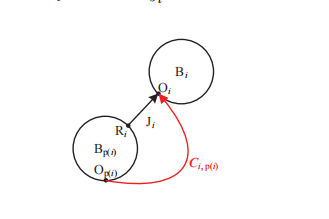
\includegraphics[width=0.8\textwidth]{Figure/PDF/SystemDynamicsModelingAndSimulation_92.png}
    \caption{牵连速度系数矩阵}
    \label{fig:chapter10_92}
\end{figure}

\paragraph{相邻体元件加速度运动学量递推关系}

将 $j$ 系相对于 $i$ 系的相对平动加速度和相对转动加速度在 $j$ 系中的六维投影列阵记为 $a_{i, j | j}$, 即

\begin{equation}
a_{i, j | j} \triangleq \begin{bmatrix}
    \bm{A}_{i, j}^T \ddot{r}_{O_i O_j | i} \\
    \dot{\omega}_{i, j | j}
\end{bmatrix},
\label{eq:10.8}
\end{equation}

相邻元件加速度运动学量递推表达式可记为

\begin{equation}
a_{0, i | i} = \bm{C}_{i, p(i)} a_{0, p(i) | p(i)} + \bm{\Phi}_{\mathrm{J}_i} \ddot{q}_{\mathrm{J}_i} + \eta_i,
\label{eq:10.9}
\end{equation}

式中

\begin{equation}
\eta_i = \xi_{\mathrm{J}_i} + \begin{bmatrix}
    \bm{A}_{p(i), i}^T \left( \tilde{\omega}_{0, p(i) | p(i)} \tilde{\omega}_{0, p(i) | p(i)} r_{O_{p(i)} O_i | p(i)} + 2 \tilde{\omega}_{0, p(i) | p(i)} \dot{r}_{O_{p(i)} O_i | p(i)} \right) \\
    \bm{A}_{p(i), i}^T \tilde{\omega}_{0, p(i) | p(i)} \omega_{p(i), i | p(i)}
\end{bmatrix},
\label{eq:10.10}
\end{equation}

式中各类铰元件相对加速度非齐次项 $\xi_{\mathrm{J}_i}$ 的具体表达式见 10.3 小节.

\section{主铰元件相对运动学方程}

\paragraph{虚拟铰元件}

对于虚拟铰元件 $i$, 位置级相对运动学方程可表示为

\begin{equation}
\begin{cases}
    r_{R_i O_i | p(i)} = l_{J_i}, \\
    \bm{A}_{p(i), i} = \bm{A}_Z(\theta_{J_i, 1}) \bm{A}_Y(\theta_{J_i, 2}) \bm{A}_X(\theta_{J_i, 3}),
\end{cases}
\label{eq:10.11}
\end{equation}

式中 $[x_{J_i}, y_{J_i}, z_{J_i}]^T =: l_{J_i}$ 和 $[\theta_{J_i, 1}, \theta_{J_i, 2}, \theta_{J_i, 3}]^T =: \theta_{J_i}$ 分别为描述虚拟铰元件 $i$ 平动和转动的广义坐标, 绕坐标轴的单位旋转矩阵表达式分别为

\begin{equation}
\bm{A}_X(\theta) = \begin{bmatrix}
    1 & 0 & 0 \\
    0 & \cos\theta & -\sin\theta \\
    0 & \sin\theta & \cos\theta
\end{bmatrix},
\bm{A}_Y(\theta) = \begin{bmatrix}
    \cos\theta & 0 & \sin\theta \\
    0 & 1 & 0 \\
    -\sin\theta & 0 & \cos\theta
\end{bmatrix},
\bm{A}_Z(\theta) = \begin{bmatrix}
    \cos\theta & -\sin\theta & 0 \\
    \sin\theta & \cos\theta & 0 \\
    0 & 0 & 1
\end{bmatrix}.
\end{equation}

速度级相对运动学方程可表示为

\begin{equation}
\begin{cases}
    \dot{r}_{R_i O_i | p(i)} = \dot{l}_{J_i}, \\
    \omega_{p(i), i | i} = \bm{H}_{B321}(\theta_{J_i}) \dot{\theta}_{J_i},
\end{cases}
\label{eq:10.12}
\end{equation}

由此可得

\begin{equation}
v_{p(i), i | i} = \begin{bmatrix}
    \bm{A}_{p(i), i}^T \dot{r}_{O_{p(i)} O_i | p(i)} \\
    \omega_{p(i), i | i}
\end{bmatrix} = \begin{bmatrix}
    \bm{A}_{p(i), i}^T \dot{r}_{R_i O_i | p(i)} \\
    \omega_{p(i), i | i}
\end{bmatrix}
= \begin{bmatrix}
    \bm{A}_{p(i), i}^T & m{O}_3 \\
    m{O}_3 & \bm{H}_{B321}(\theta_{J_i})
\end{bmatrix}
\begin{bmatrix}
    \dot{l}_{J_i} \\
    \dot{\theta}_{J_i}
\end{bmatrix}
=: \bm{\Phi}_{\mathrm{J}_i} \dot{q}_{\mathrm{J}_i}.
\label{eq:10.13}
\end{equation}

加速度相对运动学方程可表示为

\begin{equation}
\begin{cases}
    \ddot{r}_{R_i O_i | p(i)} = \ddot{l}_{J_i}, \\
    \dot{\omega}_{p(i), i | i} = \bm{H}_{B321}(\theta_{J_i}) \ddot{\theta}_{J_i} + \dot{H}_{B321}(\theta_{J_i}, \dot{\theta}_{J_i}) \dot{\theta}_{J_i},
\end{cases}
\label{eq:10.14}
\end{equation}

由此可得

\begin{equation}
a_{p(i), i | i} = \begin{bmatrix}
    \bm{A}_{p(i), i}^T \ddot{r}_{O_{p(i)} O_i | p(i)} \\
    \dot{\omega}_{p(i), i | i}
\end{bmatrix} = \begin{bmatrix}
    \bm{A}_{p(i), i}^T \ddot{r}_{R_i O_i | p(i)} \\
    \dot{\omega}_{p(i), i | i}
\end{bmatrix}
= \begin{bmatrix}
    \bm{A}_{p(i), i}^T & m{O}_3 \\
    m{O}_3 & \bm{H}_{B321}(\theta_{J_i})
\end{bmatrix}
\begin{bmatrix}
    \ddot{l}_{J_i} \\
    \ddot{\theta}_{J_i}
\end{bmatrix}
+ \begin{bmatrix}
    m{O}_3 \\
    \dot{H}_{B321}(\theta_{J_i}, \dot{\theta}_{J_i}) \dot{\theta}_{J_i}
\end{bmatrix}
=: \bm{\Phi}_{\mathrm{J}_i} \ddot{q}_{\mathrm{J}_i} + \xi_{\mathrm{J}_i}.
\label{eq:10.15}
\end{equation}

上述等式中

\begin{equation}
\bm{H}_{B321}(\theta) = \begin{bmatrix}
    -s_2 & 0 & 1 \\
    c_2 s_3 & c_3 & 0 \\
    c_2 c_3 & -s_3 & 0
\end{bmatrix},
\dot{H}_{B321} = \begin{bmatrix}
    -c_2 \dot{\theta}_2 & 0 & 0 \\
    -s_2 s_3 \dot{\theta}_2 + c_2 c_3 \dot{\theta}_3 & -s_3 \dot{\theta}_3 & 0 \\
    -s_2 c_3 \dot{\theta}_2 - c_2 s_3 \dot{\theta}_3 & -c_3 \dot{\theta}_3 & 0
\end{bmatrix},
\end{equation}

式中 $c_2 = \cos(\theta_2)$, $s_2 = \sin(\theta_2)$, $c_3 = \cos(\theta_3)$, $s_3 = \sin(\theta_3)$.

\paragraph{转动铰元件}

对于转动铰元件 $i$, 位置级相对运动学方程可表示为

\begin{equation}
\begin{cases}
    r_{R_i O_i | p(i)} = 0_3, \\
    \bm{A}_{p(i), i} = \bm{I_3} \cos\theta_{J_i} + \tilde{n}_{J_i} \sin\theta_{J_i} + \tilde{n}_{J_i} \tilde{n}_{J_i}^T (1 - \cos\theta_{J_i}) \\
    = \bm{I_3} + \tilde{n}_{J_i} \sin\theta_{J_i} + \tilde{n}_{J_i} \tilde{n}_{J_i} (1 - \cos\theta_{J_i}),
\end{cases}
\label{eq:10.16}
\end{equation}

式中 $n_{J_i}$ 表示转动铰元件 $i$ 沿转轴方向的单位矢量在 $i$ 系和 $p(i)$ 系中的投影列阵.

速度级相对运动学方程可表示为

\begin{equation}
\begin{cases}
    \dot{r}_{R_i O_i | p(i)} = 0_3, \\
    \omega_{p(i), i | i} = n_{J_i} \dot{\theta}_{J_i},
\end{cases}
\label{eq:10.17}
\end{equation}

由此可得

\begin{equation}
v_{p(i), i | i} = \begin{bmatrix}
    \bm{A}_{p(i), i}^T \dot{r}_{O_{p(i)} O_i | p(i)} \\
    \omega_{p(i), i | i}
\end{bmatrix}
= \begin{bmatrix}
    \bm{A}_{p(i), i}^T \dot{r}_{R_i O_i | p(i)} \\
    \omega_{p(i), i | i}
\end{bmatrix}
= \begin{bmatrix}
    0_3 \\
    n_{J_i}
\end{bmatrix} \dot{\theta}_{J_i}
=: \bm{\Phi}_{\mathrm{J}_i} \dot{q}_{\mathrm{J}_i}.
\label{eq:10.18}
\end{equation}

加速度相对运动学方程可表示为

\begin{equation}
\begin{cases}
    \ddot{r}_{R_i O_i | p(i)} = 0_3, \\
    \dot{\omega}_{p(i), i | i} = n_{J_i} \ddot{\theta}_{J_i},
\end{cases}
\label{eq:10.19}
\end{equation}

由此可得

\begin{equation}
a_{p(i), i | i} = \begin{bmatrix}
    \bm{A}_{p(i), i}^T \ddot{r}_{O_{p(i)} O_i | p(i)} \\
    \dot{\omega}_{p(i), i | i}
\end{bmatrix}
= \begin{bmatrix}
    \bm{A}_{p(i), i}^T \ddot{r}_{R_i O_i | p(i)} \\
    \dot{\omega}_{p(i), i | i}
\end{bmatrix}
= \begin{bmatrix}
    0_3 \\
    n_{J_i}
\end{bmatrix} \ddot{\theta}_{J_i}
=: \bm{\Phi}_{\mathrm{J}_i} \ddot{q}_{\mathrm{J}_i} + \xi_{\mathrm{J}_i}.
\label{eq:10.20}
\end{equation}

\paragraph{棱柱铰元件}

对于棱柱铰元件 $i$, 位置级相对运动学方程可表示为

\begin{equation}
\begin{cases}
    r_{R_i O_i | p(i)} = n_{J_i} l_{J_i}, \\
    \bm{A}_{p(i), i} = \bm{I_3},
\end{cases}
\label{eq:10.21}
\end{equation}

式中 $n_{J_i}$ 表示棱柱铰元件 $i$ 沿滑移轴方向的单位矢量在 $i$ 系和 $p(i)$ 系中的投影列阵.

速度级相对运动学方程可表示为

\begin{equation}
\begin{cases}
    \dot{r}_{R_i O_i | p(i)} = n_{J_i} \dot{l}_{J_i}, \\
    \omega_{p(i), i | i} = 0,
\end{cases}
\label{eq:10.22}
\end{equation}

由此可得

\begin{equation}
v_{p(i), i | i} = \begin{bmatrix}
    \bm{A}_{p(i), i}^T \dot{r}_{O_{p(i)} O_i | p(i)} \\
    \omega_{p(i), i | i}
\end{bmatrix}
= \begin{bmatrix}
    \bm{A}_{p(i), i}^T \dot{r}_{R_i O_i | p(i)} \\
    \omega_{p(i), i | i}
\end{bmatrix}
= \begin{bmatrix}
    n_{J_i} \\
    0_3
\end{bmatrix} \dot{l}_{J_i}
=: \bm{\Phi}_{\mathrm{J}_i} \dot{q}_{\mathrm{J}_i}.
\label{eq:10.23}
\end{equation}

加速度相对运动学方程可表示为

\begin{equation}
\begin{cases}
    \ddot{r}_{R_i O_i | p(i)} = n_{J_i} \ddot{l}_{J_i}, \\
    \dot{\omega}_{p(i), i | i} = 0_3,
\end{cases}
\label{eq:10.24}
\end{equation}

由此可得

\begin{equation}
a_{p(i), i | i} = \begin{bmatrix}
    \bm{A}_{p(i), i}^T \ddot{r}_{O_{p(i)} O_i | p(i)} \\
    \dot{\omega}_{p(i), i | i}
\end{bmatrix}
= \begin{bmatrix}
    \bm{A}_{p(i), i}^T \ddot{r}_{R_i O_i | p(i)} \\
    \dot{\omega}_{p(i), i | i}
\end{bmatrix}
= \begin{bmatrix}
    n_{J_i} \\
    0_3
\end{bmatrix} \ddot{l}_{J_i}
=: \bm{\Phi}_{\mathrm{J}_i} \ddot{q}_{\mathrm{J}_i} + \xi_{\mathrm{J}_i}.
\label{eq:10.25}
\end{equation}

\paragraph{固结铰元件}

对于固结铰元件 $i$, 位置级相对运动学方程可表示为

\begin{equation}
\begin{cases}
    r_{R_i O_i | p(i)} = 0_3, \\
    \bm{A}_{p(i), i} = \bm{I_3}.
\end{cases}
\label{eq:10.26}
\end{equation}

速度级相对运动学方程可表示为

\begin{equation}
\begin{cases}
    \dot{r}_{R_i O_i | p(i)} = 0_3, \\
    \omega_{p(i), i | i} = 0_3,
\end{cases}
\label{eq:10.27}
\end{equation}

由此可得

\begin{equation}
v_{p(i), i | i} = \begin{bmatrix}
    \bm{A}_{p(i), i}^T \dot{r}_{O_{p(i)} O_i | p(i)} \\
    \omega_{p(i), i | i}
\end{bmatrix}
= \begin{bmatrix}
    \bm{A}_{p(i), i}^T \dot{r}_{R_i O_i | p(i)} \\
    \omega_{p(i), i | i}
\end{bmatrix}
= \begin{bmatrix}
    0_3 \\
    0_3
\end{bmatrix}.
\label{eq:10.28}
\end{equation}

加速度相对运动学方程可表示为

\begin{equation}
\begin{cases}
    \ddot{r}_{R_i O_i | p(i)} = 0_3, \\
    \dot{\omega}_{p(i), i | i} = 0_3,
\end{cases}
\label{eq:10.29}
\end{equation}

由此可得

\begin{equation}
a_{p(i), i | i} = \begin{bmatrix}
    \bm{A}_{p(i), i}^T \ddot{r}_{O_{p(i)} O_i | p(i)} \\
    \dot{\omega}_{p(i), i | i}
\end{bmatrix}
= \begin{bmatrix}
    \bm{A}_{p(i), i}^T \ddot{r}_{R_i O_i | p(i)} \\
    \dot{\omega}_{p(i), i | i}
\end{bmatrix}
= \begin{bmatrix}
    0_3 \\
    0_3
\end{bmatrix}.
\label{eq:10.30}
\end{equation}

\paragraph{球铰元件}

对于球铰元件 $i$, 位置级相对运动学方程可表示为

\begin{equation}
\begin{cases}
    r_{R_i O_i | p(i)} = 0, \\
    \bm{A}_{p(i), i} = \bm{A}_Z(\theta_{J_i, 1}) \bm{A}_Y(\theta_{J_i, 2}) \bm{A}_X(\theta_{J_i, 3}),
\end{cases}
\label{eq:10.31}
\end{equation}

式中 $[\theta_{J_i, 1}, \theta_{J_i, 2}, \theta_{J_i, 3}]^T =: \theta_{J_i}$ 为描述球铰元件 $i$ 相对转动的广义坐标, 绕坐标轴的单位旋转矩阵表达式参见 10.3.1 小节。

速度级相对运动学方程可表示为

\begin{equation}
\begin{cases}
    \dot{r}_{R_i O_i | p(i)} = 0, \\
    \omega_{p(i), i | i} = \bm{H}_{B321}(\theta_{J_i}) \dot{\theta}_{J_i},
\end{cases}
\label{eq:10.32}
\end{equation}

由此可得

\begin{equation}
v_{p(i), i | i} = \begin{bmatrix}
    \bm{A}_{p(i), i}^T \dot{r}_{O_{p(i)} O_i | p(i)} \\
    \omega_{p(i), i | i}
\end{bmatrix} = \begin{bmatrix}
    \bm{A}_{p(i), i}^T \dot{r}_{R_i O_i | p(i)} \\
    \omega_{p(i), i | i}
\end{bmatrix}
= \begin{bmatrix}
    0_3 \\
    \bm{H}_{B321}(\theta_{J_i})
\end{bmatrix} \dot{\theta}_{J_i}
=: \bm{\Phi}_{\mathrm{J}_i} \dot{q}_{\mathrm{J}_i}.
\label{eq:10.33}
\end{equation}

\begin{equation}
=: \bm{\Phi}_{\mathrm{J}_i} \dot{q}_{\mathrm{J}_i}.
\label{eq:10.34}
\end{equation}

加速度相对运动学方程可表示为

\begin{equation}
\begin{cases}
    \ddot{r}_{R_i O_i | p(i)} = 0, \\
    \dot{\omega}_{p(i), i | i} = \bm{H}_{B321}(\theta_{J_i}) \ddot{\theta}_{J_i} + \dot{H}_{B321}(\theta_{J_i}, \dot{\theta}_{J_i}) \dot{\theta}_{J_i},
\end{cases}
\label{eq:10.35}
\end{equation}

由此可得

\begin{equation}
a_{p(i), i | i} = \begin{bmatrix}
    \bm{A}_{p(i), i}^T \ddot{r}_{O_{p(i)} O_i | p(i)} \\
    \dot{\omega}_{p(i), i | i}
\end{bmatrix} = \begin{bmatrix}
    \bm{A}_{p(i), i}^T \ddot{r}_{R_i O_i | p(i)} \\
    \dot{\omega}_{p(i), i | i}
\end{bmatrix}
= \begin{bmatrix}
    0_3 \\
    \bm{H}_{B321}(\theta_{J_i})
\end{bmatrix} \ddot{\theta}_{J_i}
+ \begin{bmatrix}
    0_3 \\
    \dot{H}_{B321}(\theta_{J_i}, \dot{\theta}_{J_i}) \dot{\theta}_{J_i}
\end{bmatrix}
=: \bm{\Phi}_{\mathrm{J}_i} \ddot{q}_{\mathrm{J}_i} + \xi_{\mathrm{J}_i}.
\label{eq:10.36}
\end{equation}

上述等式中 $\bm{H}_{B321}$ 和 $\dot{H}_{B321}$ 的具体表达式详见 10.3.1 小节.

\paragraph{万向节}

\paragraph{圆柱铰}

\paragraph{螺旋铰}

\section{体元件速度关于系统广义速度的线性表达式}

对于任意体元件 $i$, 其绝对速度列阵 $v_{0, i | i}$ 可记为如下形式

\begin{equation}
v_{0, i | i} = \sum_{k \in \bar{p}[i]} \bm{C}_{i, k} \bm{\Phi}_{\mathrm{J}_k} \dot{q}_{\mathrm{J}_k},
\label{eq:10.37}
\end{equation}

式中牵连速度矩阵

\begin{equation}
\bm{C}_{i, k} = \begin{bmatrix}
    \bm{A}_{k, i}^T & \bm{A}_{k, i}^T \tilde{r}_{O_k O_i | k} \\
    m{O}_3 & \bm{A}_{k, i}^T
\end{bmatrix}, \quad k \in \bar{p}[i],
\label{eq:10.38}
\end{equation}

当 $k = p(i)$ 时, 有

\begin{equation}
\bm{C}_{i, p(i)} = \begin{bmatrix}
    \bm{A}_{p(i), i}^T & \bm{A}_{p(i), i}^T \tilde{r}_{O_{p(i)} O_i | p(i)} \\
    m{O}_3 & \bm{A}_{p(i), i}^T
\end{bmatrix},
\label{eq:10.39}
\end{equation}

该表达式与式~\eqref{eq:10.7} 相同； 当 $k = i$ 时, 有

\begin{equation}
\bm{C}_{i, i} = \begin{bmatrix}
    \bm{A}_{i, i}^T & \bm{A}_{i, i}^T \tilde{r}_{O_i O_i | i} \\
    m{O}_3 & \bm{A}_{i, i}^T
\end{bmatrix} = \begin{bmatrix}
    \bm{I_3} & m{O}_3 \\
    m{O}_3 & \bm{I_3}
\end{bmatrix} = \bm{I_6}.
\label{eq:10.40}
\end{equation}

对于任意元件 $i$, 其牵连速度系数矩阵 (10.38) 满足如下递推规律 (运算量较大)

\begin{equation}
\bm{C}_{i, k} = \begin{cases}
    \bm{I_6} & k = i, \\
    \bm{C}_{i, p(i)} C_{p(i), k} & k \in \bar{p}[\bar{p}[i]].
\end{cases}
\label{eq:10.41}
\end{equation}

\begin{figure}[H]
    \centering
    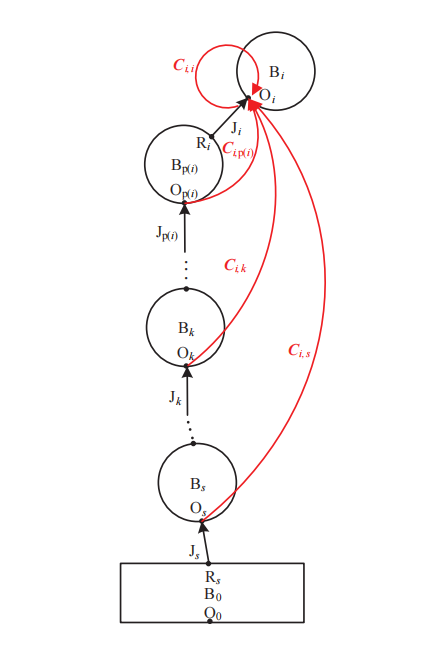
\includegraphics[width=0.8\textwidth]{Figure/PDF/SystemDynamicsModelingAndSimulation_100.png}
    \caption{体元件前序元件牵连速度系数矩阵}
    \label{fig:chapter10_100}
\end{figure}

\section{闭环切断铰元件相对运动学量的计算}

系统闭环切断铰元件相对运动学量并未作为系统广义坐标的一部分, 需借助当前时刻的系统广义坐标来确定, 计算过程中有时也要综合考虑该切断铰上一时刻的相对运动学量, 以防计算结果发生突变.

\paragraph{转动铰元件}

当 $L_j$ 为转动铰时, 动系到基系的坐标转换矩阵可表示为

\begin{equation}
\bm{A}_{\underline{b}(j), \underline{m}(j)} = \bm{I_3} \cos\theta_{L_i} + \tilde{n}_{L_i} \sin\theta_{L_i} + n_{L_i} n_{L_i}^T (1 - \cos\theta_{L_i})
= \begin{bmatrix}
    a_{11} & a_{12} & a_{13} \\
    a_{21} & a_{22} & a_{23} \\
    a_{31} & a_{32} & a_{33}
\end{bmatrix}_{\underline{b}(j), \underline{m}(j)}.
\label{eq:10.42}
\end{equation}

由此可得

\begin{equation}
\text{tr} \bm{A}_{\underline{b}(j), \underline{m}(j)} = 1 + 2 \cos\theta_{L_i}
\label{eq:10.43}
\end{equation}

和

\begin{equation}
2 n_{L_i} \sin\theta_{L_i} = \begin{bmatrix}
    a_{32} - a_{23} \\
    a_{13} - a_{31} \\
    a_{21} - a_{12}
\end{bmatrix}_{\underline{b}(j), \underline{m}(j)}.
\label{eq:10.44}
\end{equation}

由以上两式进一步可得

\begin{equation}
\cos\theta_{L_i} = \frac{\text{tr} \bm{A}_{\underline{b}(j), \underline{m}(j)} - 1}{2} =: X
\label{eq:10.45}
\end{equation}

和

\begin{equation}
\sin\theta_{L_i} = \frac{1}{2} n_{L_i}^T \begin{bmatrix}
    a_{32} - a_{23} \\
    a_{13} - a_{31} \\
    a_{21} - a_{12}
\end{bmatrix}_{\underline{b}(j), \underline{m}(j)} =: Y.
\label{eq:10.46}
\end{equation}

在 $(-\pi, \pi]$ 区间内可得

\begin{equation}
\hat{\theta}_{L_i} = \text{atan2}(Y, X).
\label{eq:10.47}
\end{equation}

将上一时刻 $L_j$ 的转角记为

\begin{equation}
\theta_{L_i}^- = \hat{\theta}_{L_i}^- + 2\pi N_{L_i}^-,
\label{eq:10.48}
\end{equation}

式中 $\hat{\theta}_{L_i}^- \in (-\pi, \pi]$, $N_{L_i}^- \in \mathbb{N}$. 则当前时刻运动学量满足

\begin{equation}
\hat{\theta}_{L_i}^+ = \hat{\theta}_{L_i},
\label{eq:10.49}
\end{equation}

\begin{equation}
N_{L_i}^+ = \begin{cases}
    N_{L_i}^- + 1, & \hat{\theta}_{L_i}^- > \pi/2 \quad \text{and} \quad \hat{\theta}_{L_i} < -\pi/2, \\
    N_{L_i}^- - 1, & \hat{\theta}_{L_i}^- < -\pi/2 \quad \text{and} \quad \hat{\theta}_{L_i} > \pi/2,
\end{cases}
\label{eq:10.50}
\end{equation}

\begin{equation}
\theta_{L_i} = \hat{\theta}_{L_i}^+ + 2\pi N_{L_i}^+.
\label{eq:10.51}
\end{equation}

\paragraph{棱柱铰元件}

\paragraph{固结铰元件}

\paragraph{球铰元件}

\paragraph{万向节}

\section{闭环切断铰元件约束方程}

\paragraph{转动铰元件}

当闭环 $L_j$ 切断铰为转动铰元件时, 其位置级约束方程可表示为

\begin{equation}
0 = c_{L_j} = \begin{bmatrix}
    r_{O_{\underline{f}(j)} M_j | \underline{f}(j)} - r_{O_{\underline{f}(j)} B_j | \underline{f}(j)} \\
    \bm{T}_{L_j}^T \bm{A}_{\underline{f}(j), \underline{b}(j)}^T \bm{A}_{\underline{f}(j), \underline{m}(j)} n_{L_j}
\end{bmatrix} =: \begin{bmatrix}
    c_{L_j, U} \\
    c_{L_j, D}
\end{bmatrix},
\label{eq:10.52}
\end{equation}

式中

\begin{equation}
r_{O_{\underline{f}(j)} M_j | \underline{f}(j)} = r_{O_{\underline{f}(j)} O_{\underline{m}(j)} | \underline{f}(j)} + \bm{A}_{\underline{f}(j), \underline{m}(j)} r_{O_{\underline{m}(j)} M_j | \underline{m}(j)},
\label{eq:10.53}
\end{equation}

\begin{equation}
r_{O_{\underline{f}(j)} B_j | \underline{f}(j)} = r_{O_{\underline{f}(j)} O_{\underline{b}(j)} | \underline{f}(j)} + \bm{A}_{\underline{f}(j), \underline{b}(j)} r_{O_{\underline{b}(j)} B_j | \underline{b}(j)},
\label{eq:10.54}
\end{equation}

三维列阵 $n_{L_j}$ 为在 $\underline{b}(j)$ 系和 $\underline{m}(j)$ 系中表示的切断铰转轴方向的单位矢量. $\bm{T}_{L_j} = [\tau_{L_j, 1} \quad \tau_{L_j, 2}]$, $\tau_{L_j, 1}$ 和 $\tau_{L_j, 2}$ 为建模时定义的一对模为 1 的定常三维列阵; $\tau_{L_j, 1}$, $\tau_{L_j, 2}$ 与 $n_{L_j}$ 两两正交.

位置级约束方程中 $c_{L_j, U}$ 关于时间的一阶导数满足

\begin{align}
\dot{c}_{L_j, U} &= \dot{r}_{O_{\underline{f}(j)} M_j | \underline{f}(j)} - \dot{r}_{O_{\underline{f}(j)} B_j | \underline{f}(j)} \notag \\
&= \frac{d}{dt} \left( r_{O_{\underline{f}(j)} O_{\underline{m}(j)} | \underline{f}(j)} + \bm{A}_{\underline{f}(j), \underline{m}(j)} r_{O_{\underline{m}(j)} M_j | \underline{m}(j)} \right) \notag \\
&\quad - \frac{d}{dt} \left( r_{O_{\underline{f}(j)} O_{\underline{b}(j)} | \underline{f}(j)} + \bm{A}_{\underline{f}(j), \underline{b}(j)} r_{O_{\underline{b}(j)} B_j | \underline{b}(j)} \right) \notag \\
&= \dot{r}_{O_{\underline{f}(j)} O_{\underline{m}(j)} | \underline{f}(j)} + \bm{A}_{\underline{f}(j), \underline{m}(j)} \tilde{\omega}_{\underline{f}(j), \underline{m}(j) | \underline{m}(j)} r_{O_{\underline{m}(j)} M_j | \underline{m}(j)} \notag \\
&\quad - \dot{r}_{O_{\underline{f}(j)} O_{\underline{b}(j)} | \underline{f}(j)} - \bm{A}_{\underline{f}(j), \underline{b}(j)} \tilde{\omega}_{\underline{f}(j), \underline{b}(j) | \underline{b}(j)} r_{O_{\underline{b}(j)} B_j | \underline{b}(j)} \notag \\
&= \bm{A}_{\underline{f}(j), \underline{m}(j)} \bm{A}_{\underline{f}(j), \underline{m}(j)}^T \dot{r}_{O_{\underline{f}(j)} O_{\underline{m}(j)} | \underline{f}(j)}
+ \bm{A}_{\underline{f}(j), \underline{m}(j)} \tilde{r}_{O_{\underline{m}(j)} M_j | \underline{m}(j)}^T \omega_{\underline{f}(j), \underline{m}(j) | \underline{m}(j)} \notag \\
&\quad - \bm{A}_{\underline{f}(j), \underline{b}(j)} \bm{A}_{\underline{f}(j), \underline{b}(j)}^T \dot{r}_{O_{\underline{f}(j)} O_{\underline{b}(j)} | \underline{f}(j)}
- \bm{A}_{\underline{f}(j), \underline{b}(j)} \tilde{r}_{O_{\underline{b}(j)} B_j | \underline{b}(j)}^T \omega_{\underline{f}(j), \underline{b}(j) | \underline{b}(j)} \notag \\
&= \left[ \bm{A}_{\underline{f}(j), \underline{m}(j)} \quad \bm{A}_{\underline{f}(j), \underline{m}(j)} \tilde{r}_{O_{\underline{m}(j)} M_j | \underline{m}(j)}^T \right] \begin{bmatrix}
    \bm{A}_{\underline{f}(j), \underline{m}(j)}^T \dot{r}_{O_{\underline{f}(j)} O_{\underline{m}(j)} | \underline{f}(j)} \\
    \omega_{\underline{f}(j), \underline{m}(j) | \underline{m}(j)}
\end{bmatrix} \notag \\
&\quad - \left[ \bm{A}_{\underline{f}(j), \underline{b}(j)} \quad \bm{A}_{\underline{f}(j), \underline{b}(j)} \tilde{r}_{O_{\underline{b}(j)} B_j | \underline{b}(j)}^T \right] \begin{bmatrix}
    \bm{A}_{\underline{f}(j), \underline{b}(j)}^T \dot{r}_{O_{\underline{f}(j)} O_{\underline{b}(j)} | \underline{f}(j)} \\
    \omega_{\underline{f}(j), \underline{b}(j) | \underline{b}(j)}
\end{bmatrix} \notag \\
&=: \left[ \bm{A}_{\underline{f}(j), \underline{m}(j)} \quad \bm{A}_{\underline{f}(j), \underline{m}(j)} \tilde{r}_{O_{\underline{m}(j)} M_j | \underline{m}(j)}^T \right] v_{\underline{f}(j), \underline{m}(j) | \underline{m}(j)} \notag \\
&\quad - \left[ \bm{A}_{\underline{f}(j), \underline{b}(j)} \quad \bm{A}_{\underline{f}(j), \underline{b}(j)} \tilde{r}_{O_{\underline{b}(j)} B_j | \underline{b}(j)}^T \right] v_{\underline{f}(j), \underline{b}(j) | \underline{b}(j)}. \label{eq:10.55}
\end{align}

位置级约束方程中 $c_{L_j, D}$ 关于时间的一阶导数满足

\begin{align}
\dot{c}_{L_j, D} &= \frac{d}{dt} \left( \bm{T}_{L_j}^T \bm{A}_{\underline{f}(j), \underline{b}(j)}^T \bm{A}_{\underline{f}(j), \underline{m}(j)} n_{L_j} \right) \notag \\
&= \bm{T}_{L_j}^T \dot{\bm{A}}_{\underline{f}(j), \underline{b}(j)}^T \bm{A}_{\underline{f}(j), \underline{m}(j)} n_{L_j} + \bm{T}_{L_j}^T \bm{A}_{\underline{f}(j), \underline{b}(j)}^T \dot{\bm{A}}_{\underline{f}(j), \underline{m}(j)} n_{L_j} \notag \\
&= \bm{T}_{L_j}^T \bm{A}_{\underline{f}(j), \underline{b}(j)}^T \tilde{\omega}_{\underline{f}(j), \underline{b}(j) | \underline{b}(j)} \bm{A}_{\underline{f}(j), \underline{m}(j)} n_{L_j} - \bm{T}_{L_j}^T \bm{A}_{\underline{f}(j), \underline{b}(j)}^T \tilde{\omega}_{\underline{f}(j), \underline{m}(j) | \underline{m}(j)} \bm{A}_{\underline{f}(j), \underline{m}(j)} n_{L_j} \notag \\
&= \bm{T}_{L_j}^T \bm{A}_{\underline{f}(j), \underline{b}(j)}^T \bm{A}_{\underline{f}(j), \underline{m}(j)} \tilde{n}_{L_j} \omega_{\underline{f}(j), \underline{b}(j) | \underline{b}(j)} - \bm{T}_{L_j}^T \bm{A}_{\underline{f}(j), \underline{b}(j)}^T \bm{A}_{\underline{f}(j), \underline{m}(j)} \tilde{n}_{L_j} \omega_{\underline{f}(j), \underline{m}(j) | \underline{m}(j)} \notag \\
&= \bm{T}_{L_j}^T \bm{A}_{\underline{b}(j), \underline{m}(j)} \tilde{n}_{L_j} \omega_{\underline{f}(j), \underline{b}(j) | \underline{m}(j)} - \bm{T}_{L_j}^T \bm{A}_{\underline{b}(j), \underline{m}(j)} \tilde{n}_{L_j} \omega_{\underline{f}(j), \underline{m}(j) | \underline{m}(j)} \notag \\
&= \bm{T}_{L_j}^T \bm{A}_{\underline{b}(j), \underline{m}(j)} \tilde{n}_{L_j} \bm{A}_{\underline{b}(j), \underline{m}(j)}^T \omega_{\underline{f}(j), \underline{b}(j) | \underline{b}(j)} - \bm{T}_{L_j}^T \bm{A}_{\underline{b}(j), \underline{m}(j)} \tilde{n}_{L_j} \omega_{\underline{f}(j), \underline{m}(j) | \underline{m}(j)} \notag \\
&= \left[ \bm{O}_{2 \times 3} \quad \bm{T}_{L_j}^T \bm{A}_{\underline{b}(j), \underline{m}(j)} \tilde{n}_{L_j}^T \right] \begin{bmatrix}
    \bm{A}_{\underline{f}(j), \underline{m}(j)}^T \dot{r}_{O_{\underline{f}(j)} O_{\underline{m}(j)} | \underline{f}(j)} \\
    \omega_{\underline{f}(j), \underline{m}(j) | \underline{m}(j)}
\end{bmatrix} \notag \\
&\quad - \left[ \bm{O}_{2 \times 3} \quad \bm{T}_{L_j}^T \bm{A}_{\underline{b}(j), \underline{m}(j)} \tilde{n}_{L_j} \bm{A}_{\underline{b}(j), \underline{m}(j)}^T \right] \begin{bmatrix}
    \bm{A}_{\underline{f}(j), \underline{b}(j)}^T \dot{r}_{O_{\underline{f}(j)} O_{\underline{b}(j)} | \underline{f}(j)} \\
    \omega_{\underline{f}(j), \underline{b}(j) | \underline{b}(j)}
\end{bmatrix} \notag \\
&= \left[ \bm{O}_{2 \times 3} \quad \bm{T}_{L_j}^T \bm{A}_{\underline{b}(j), \underline{m}(j)} \tilde{n}_{L_j}^T \right] v_{\underline{f}(j), \underline{m}(j) | \underline{m}(j)} \notag \\
&\quad - \left[ \bm{O}_{2 \times 3} \quad \bm{T}_{L_j}^T \bm{A}_{\underline{b}(j), \underline{m}(j)} \tilde{n}_{L_j} \bm{A}_{\underline{b}(j), \underline{m}(j)}^T \right] v_{\underline{f}(j), \underline{b}(j) | \underline{b}(j)}. \label{eq:10.57}
\end{align}

当闭环 $L_j$ 切断铰为转动铰元件时, 则有

\begin{equation}
\dot{c}_{L_j} = \begin{bmatrix}
    \dot{c}_{L_j, U} \\
    \dot{c}_{L_j, D}
\end{bmatrix}
= \begin{bmatrix}
    \bm{A}_{\underline{f}(j), \underline{m}(j)} & \bm{A}_{\underline{f}(j), \underline{m}(j)} \tilde{r}_{O_{\underline{m}(j)} M_j | \underline{m}(j)}^T \\
    \bm{O}_{2 \times 3} & \bm{T}_{L_j}^T \bm{A}_{\underline{b}(j), \underline{m}(j)} \tilde{n}_{L_j}^T
\end{bmatrix} v_{\underline{f}(j), \underline{m}(j) | \underline{m}(j)}
- \begin{bmatrix}
    \bm{A}_{\underline{f}(j), \underline{b}(j)} & \bm{A}_{\underline{f}(j), \underline{b}(j)} \tilde{r}_{O_{\underline{b}(j)} B_j | \underline{b}(j)}^T \\
    \bm{O}_{2 \times 3} & \bm{T}_{L_j}^T \bm{A}_{\underline{b}(j), \underline{m}(j)} \tilde{n}_{L_j} \bm{A}_{\underline{b}(j), \underline{m}(j)}^T
\end{bmatrix} v_{\underline{f}(j), \underline{b}(j) | \underline{b}(j)}
=: \bm{\Psi}_{\underline{m}(j)} v_{\underline{f}(j), \underline{m}(j) | \underline{m}(j)} - \bm{\Psi}_{\underline{b}(j)} v_{\underline{f}(j), \underline{b}(j) | \underline{b}(j)}.
\label{eq:10.58}
\end{equation}

\paragraph{棱柱铰元件}

\paragraph{固结铰元件}

\paragraph{球铰元件}

\paragraph{万向节}